\chapter{Related Work}
\label{cha:related_work}

Path planning is a fundamental problem, so it is unsurprising that there are already many possible solutions. Several well-known algorithms have been used to tackle this problem or combined in order to achieve better results. However, it is also a very complex problem and has been shown to be PSPACE-hard \cite{39}, with its complexity growing exponentially with the configuration space, in our case the number of trailers. \cite{1} In the following chapter we will take a closer look at some of the solutions proposed and also consider their complexity and their problems with this particular task. This chapter is split in two parts, the first one concentrating on incremental algorithms and probabilistic metaheuristics, the second one instead focusing on other machine learning approaches. The focus in either case is the usefulness of the algorithm as a path-planning solution for a general-n-trailer. \pagebreak[4]

\section{Common Path-Planning Algorithms}
\label{sec:common_pathplanning}

In order to use the algorithms presented here we have to construct a configuration space (C-space), which is achieved by representing any possible configuration, that is direction and position of all elements of the vehicle, as a single point in this C-space. The size of this C-space is one of the biggest factors in the algorithms performance, it is determined by two factors: The number of degrees of freedom our system has, in this case the number of trailers, as well as the magnitude of our grid with which we overlay the map with in order to allow orientation. This magnitude depends on both the size of our map as well as the chosen resolution.

\subsection{Rapidly-exploring Random Tree}
\label{sec:rrt}

Rapidly-exploring Random Trees (RRT)\cite{40} are an efficient method for path-planning in high dimensional spaces, including cases such as ours, where nonholonomic constraints are given.\cite{33,34} It works by randomly choosing a configuration (or, if a collision detection is given, a free configuration) from the configuration space C and then looking for a vertex in the tree that is close to the chosen configuration. Then it moves a distance $\detla q$ in direction of that target configuration, taking movement constraints into account. The now reached configuration $q_(new)$, which is close to the initially randomly chosen target configuration, is then added to the RRT and the process is repeated. This algorithm can be started simultaneously from several points of the map, for example the start and target position, and then try to meet the other tree to gain a continuous path through the map. While RRTs can produce paths through complex environments quickly, even while taking different constraints into account, it is not a sufficient path-planning algorithm when used alone. The resulting paths are suboptimal and contain a large number of needles turns and sharp corners. An optimization algorithm is required to flatten the path and make it a more feasible solution. It is however a good way to quickly find a path at all, using a different algorithm for optimization later can still result in an overall better performance than comparable algorithms. 

\subsection{Path Transformation}
\label{sec:pathtransformation}

Path transformation is a simple way to find a path in a grid-based environment (see \ref{sec:a_star}) and combines two other transformations: distance- and obstacle transformation \cite{35}. Distance transformation works by assigning every cell of the grid a value which represents the distance from this cell to the target cell, see fig. \ref{pic:distance_transformation} for an example. How this distance is computed depends on the chosen movement model, basically whether we choose that our vehicle can move diagonally for the same cost as horizontally/vertically, a higher cost, or not at all. The later case meaning moving diagonally has twice the cost of horizontally/vertically since it is seen as a combination of two such moves. If a map has been updated with such values a path can easily be found simply by always choosing a cell with a lower value as the next step. The costs of the entire path is also clear from the beginning since it is stated in the first cell. Obstacle transformation works similarly by assigning each cell a value stating the distance between this cell and the closest obstacle as can be seen in fig. \ref{pic:obstacle_transformation}. Path transformation now combines both these maps under a certain weighting which states whether the length or the safety of the path is more important. Avoiding cells with low obstacle value is safer while avoiding cells with high distance value is shorter, so by adjusting this weighting a balance between safety and distance can be found. 
While path transformation is a simple and often used way to find a path, it is not well suited to high dimensional problems with nonholonomic constraints such as our case here. Its efficiency also heavily depends on the chosen resolution of the map.

\begin{figure}[b]
\centering
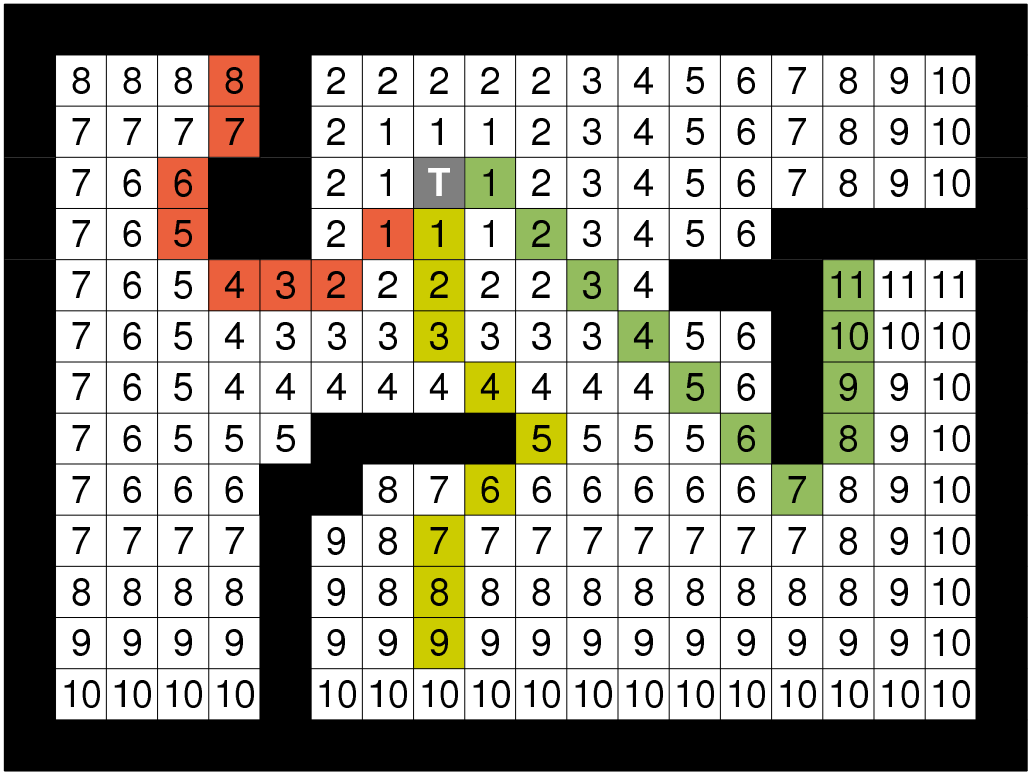
\includegraphics[width=0.75\textwidth]{./Chapters/Figures/distance_transformation.png}
\caption{A map filled with distance transformation values\label{pic:distance_transformation}}
\end{figure}

\begin{figure}[b]
\centering
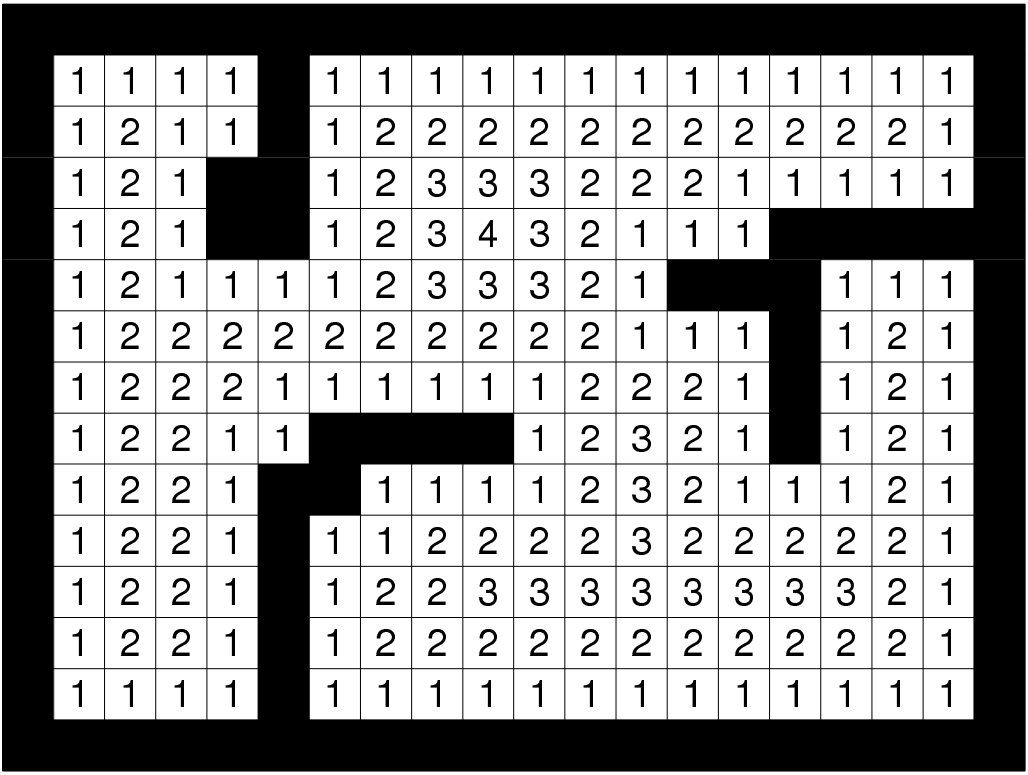
\includegraphics[width=0.75\textwidth]{./Chapters/Figures/obstacle_transformation.png}
\caption{A map filled with obstacle transformation values\label{pic:obstacle_transformation}}
\end{figure}

\section{Algorithms for Graph-Based Path-Planning}
\label{sec:graphbased_pathplanning}

In order to plan a path using incremental algorithms we first have to convert our path planning into a graph searching problem. To this end we have to construct a suitable graph from a given C-space. There are several approaches to this task, for example the visibility graph approach \cite{2,3} and the retraction method \cite{4,5}, but for the purpose of this paper it is enough to know that such a conversion into a graph searching problem is possible. 

\subsection{A* Algorithm}
\label{sec:a_star}

The A* algorithm is one of the most widespread solutions for graph traversal problems.\cite{8} In order to utilize it for motion planning the area has to be overlaid with a configuration space and then transformed into a graph as described above. This leads to several problems for our path planning task. The complexity of the problem depends on the size of the graph, which in turn depends on the size of the configuration space. A finer grid leads to a larger number of vertices in the graph and, as the computation time of the A* algorithm grows exponentially with this number, results in slower performance. However, a coarse grid would ignore possible paths since obstacles would appear greater than they are. To a certain point this can be useful to prevent collisions, but it also means a loss of information and consequently fewer options to choose from, possibly missing better paths. There may also be additional constraints the path has to satisfy, which further slow down computation. So while A*, or similar graph searching algorithms, like Dijkstra's graph search \cite{6}, can be used, their performance for this kind of complex problem prevents them from being feasible.

\subsection{Hill Climbing}
\label{sec:hill_climbing}

Another common algorithm used to tackle graph searching problems is hill climbing. It is popular due to it's simplicity and ability to find a local optimum in a short amount of time, also it can return a result an any point, even when it is not yet finished. This may be relevant in real-time system, where it is more important to have a solution at a given time than to have an optimized solution later. This may also hold true for motion planning task, when the speed of planning is more important than the quality of the resulting path. In our given case however the quality of the path is more important than the speed of computation. In simple cases, Hill Climbing produces paths of similar quality when compared to simulated annealing or genetic algorithms \cite{8}, however as the search space grows more complex, the algorithm fails to generate good solutions. This is due to its very local searching behaviour which becomes more of an obstacle the larger the search space gets. Various optimization techniques try to mitigate this problem, such as stochastic hill climbing, \label{sec:stochastic_hill_climbing} which does not examine all neighbours but chooses randomly and then evaluates whether to move there or to examine another one, or random-restart hill climbing, which tries to counter the locality issue by choosing its start point at random and then repeat the entire search several times. Even with these optimizations in place, hill climbing still cannot compete with other algorithms in solving problems of the complexity we consider here. Stochastic hill climbing produces paths similar to standard hill climbing at equal or even greater cost \cite{8} and also fails to produce good results once the search space becomes too large. Random-restart hill climbing could potentially produce good results, but in a large search space this would very much rely on luck. Since the algorithm would have to run many times to have at least some chance of finding a globally good path the performance would suffer greatly. Also, unlike A*, hill climbing can never guarantee that the optimal path has been found, this however is also true for our machine learning algorithms.

\subsection{Simulated Annealing}
\label{sec:simulated_annealing}

Simulated Annealing is a probabilistic metaheuristic which searches for an optimum solution in a way similar to hill climbing, that is, by always considering the neighbours of the current position and then using a given function to determine whether or not to move to that neighbour. Unlike hill climbing however, simulated annealing changes its behaviour over time, according to a global parameter $T$ (Temperature). $T$ can be defined freely, but always ends with $T=0$. Every state is assigned an energy $e$ which is smaller the better the state is. The algorithm favours moves that go towards lower energy states the smaller $T$ is, so it starts out by ignoring local minima and moves loosely towards areas that contain good solutions overall. Then, with lower $T$, it starts preferring moves that go "`downhill"', meaning towards lower energy states, more so that it starts moving towards the local minimum in the given region once $T$ gets close to $0$. Due to this, simulated annealing circumvents the hill climbing problem of solely moving towards local solutions while ignoring the global ones. The algorithm shows results similar to those of a genetic algorithms, but is significantly outperformed as far as number evaluation is concerned.\cite{8}

% Iterative Algorithms End

\section{Alternative Machine Learning Algorithms for Path-Planning}
\label{sec:alternative_machine_learning_pathplanning}

As we can see from the algorithms presented in \ref{sec:alternative_pathplanning} an iterative approach causes a number of problems when it comes to complex tasks. Since we want to develop a solution for a general-n-trailer, with theoretically infinite degrees of freedom, an algorithm that stops producing feasible results for non-trivial problems is not an option. Of the five algorithms presented, simulated annealing is the only one that produces useful results, but also requires a very large number of computations \cite{8} for more complex problems. In order to avoid these issues, a number of machine learning algorithms have been proposed to solve the motion planning problem. In the following section we will consider four of these approaches, including a second implementation of the genetic algorithm (GA). This GA is important since the comparisons to hill climbing and simulated annealing referred to earlier have been made using that implementation and not the one developed in this paper. \cite{8}

\subsection{Reinforced Learning}
\label{sec:reinforced_learning}

Reinforced Learning is one category of machine learning algorithms with different capabilities depending on the method used. Before focusing further on any of these specific algorithms, a general overview of the principles of reinforced learning will be given. The general idea of reinforced learning is to assign a certain reward to any action. This reward can be positive or negative (punishment) and its value depends on the action taken. The task of the algorithm is to choose a path through this graph such that the accumulated reward at the end is maximal. Since always choosing the greater reward at any point obviously does not mean achieving the greatest accumulated reward, a balance between exploration and exploitation has to be found. Exploitation means picking the best choice available in the current state and exploration means picking sub optimal choices in the hopes that actions further down this part of the decision tree are overall better. To this end an $\epsilon$-greedy algorithm with an $\epsilon$ value of $5\%$ is usually used, where a greater $\epsilon$ value means more exploration and a smaller value infers more exploitation. For path planning tasks a Markov process is usually assumed, which means that only current inputs, in our case the current position of the truck, are considered and past ones are ignored. This means that old inputs do not have to be stored, so no memory is required for that, and computation becomes much simpler since fewer variables are considered. Reinforced learning algorithms can be split into three groups depending on their model of the environment and their bootstrapping capability. Bootstrapping means that estimates are updated based on other estimates, which speeds up the algorithm. These three groups are dynamic programming methods (DP), monte carlo methods (MC) and temporal difference methods (TD). MC and TD don't need an exact model of the environment, where MC uses no bootstrapping but TD does. DP also uses bootstrapping but needs an exact model of the environment, which makes it less feasible for motion-planning purposes.
\cite{9}. Specific reinforced learning implementations can be categorized according to these three methods. Both TD and MC methods can be split further depending on whether they are on-policy or off-policy, where on-policy uses a first-visit method, where the value of a state-action pair is determined be the average return after the first instance of a given state. Because there is no guarantee that all state-action pairs will be visited, on policy is $\epsilon$-greedy so it approaches an optimal policy while still maintaining exploration. In our case this simply means that we have an $\epsilon$ chance of selection a random action rather than the best action. Off-policy separates the evaluation policy into behaviour and estimation policy. It follows the behaviour policy while it evaluates and improves the estimation policy. Due to this separation, $\epislon$-greedy is not needed to evaluate all state-action pairs, however, since the learning rate for greedy and non-greedy actions are different the algorithm is slower for some states. 
In the following we will now have a closer look at three such algorithms.

\subsubsection{Q-Learning}
\label{sec:q-learning}

Q-Learning is an off-policy, $\epsilon$-greedy TD method which learns an action-value function independent from the given policy to make an assumption about the optimal policy. Compared to other algorithms it is exploration heavy and will probably make more random decisions than exploitative decisions, due to this it is also more likely to find the optimal policy in a finite number amount of time. Q-Learning requires the actions and states to be defined. In our case states are sensor data, or our current position, and actions are basic movement actions, here left/right in a certain angle and forward driving. Since reinforced learning takes a large number of samples to learn from, the first step should be done in a simulation, similar to the one developed for the evaluation of our genetic algorithm. Simulations have the downside of being inaccurate since a model can never represent the real world perfectly, but can in turn be used much easier and much more quickly. Also data from a simulation can be stored and evaluated easily and the process can simply be automated. Once an optimal policy has been found using the simulation it has to be further refined using the actual vehicle. Depending on the accuracy of the simulation this will only require a small number of episodes. This phase may still be the most time consuming however since it cannot be sped up like the simulation. Depending on the vehicle and space required for the task, in our case a parking space and a truck, this task will still be the most challenging.

\subsubsection{Extended Q-Learning}
\label{sec:extended-q-learning}
Classical Q-Learning needs to make $m-1$ comparisons to maximize the Q-value in a given state, so assuming n states the overall time-complexity of Q-Learning is $\mathcal O(n(m-1))$. This can be optimized by using extended Q-Learning \cite{11}. We introduce an additional variable, $L_x$, for each state. $L_x$ is a lock bit and is 1 if the value $Q_x$ of the state $S_x$ is locked and won't be updated further, or 0 otherwise. At the beginning we have $L_n=0$ for all $S_n$ except the goal state. There are a number of properties that can be used to quickly set $L_n$ throughout the algorithm's run time: 

\vspace{1\baselineskip}\vspace{-\parskip}

\begin{flushleft}
Property 1: If $L_n=1$ and $d_p_G > d_n_G$ then $Q_p = \gamma \times Q_n$ and set $L_p=1$\\
Property 2: If $L_n=0$ and $d_p_G > d_n_G$ then $Q_p = Max(Q_p,\gamma \times Q_n)$\\
Property 3: If $L_n=1$ and $d_n_G > d_p_G$ then $Q_n = \gamma \times Q_p$ and set $L_n=1$\\
Property 4: If $L_n=0$ and $d_n_G > d_p_G$ then $Q_n = Max(Q_n,\gamma \times Q_p)$\\
\end{flushleft}

\vspace{1\baselineskip}\vspace{-\parskip}

Using these properties, both $L_i$ and $Q_i$ can be updated accordingly. Now, in order to determine if a state is optimal, we only need to check whether or not it is locked. So for $n$ states we only need $n$ comparisons, so we save $\mathcal O(n(m-1)-n=nm-2n=n(m-2))$ \cite{11} comparisons.
For space complexity we previously had $n \times m $ for classical Q-Learning whereas we only need $3$ values for any state in the extended Q-Learning algorithm: Q-Value, $L_x$ and the best action at that state. This means a space-complexity of only $3 \times n$ and a saving of $\mathcal O(nm-3n=n(m-3))$.\cite{11}


% \subsubsection{R-Learning}
% \label{sec:r-learning}

% \subsubsection{Sarsa}
% \label{sec:sarsa}

% \subsubsection{Actor-critic}
% \label{sec:actor-critic}

%\subsection{Genetic Algorithm}
%\label{sec:genetic_algorithm}

%In this section we will cover the genetic algorithm (GA) proposed by Andreas C. Nearchou \cite{8} as a comparison to the iterative algorithms covered in \ref{sec:alternative_pathplanning}. For a general description of the GA refer to \ref{sec:previous_knowledge_ga} and for an in-depth implementation of the GA developed for this paper refer to \ref{cha:algorithm_details}.
%The genome in this case is represented as a bit string of the length of the path where each bit represents a vertex in the graph and marks whether or not it is part of the solution. The first bit marks the first vertex, the $N$th bit the last vertex. The initial generation is obtained by randomly choosing a path length and then flipping a fair coin to decide whether any vertex on the graph is taken or not. This includes impossible paths that would collide with an obstacle, these are then filtered out by the fitness function. In addition, paths get a better rating depending the total weight of their vertices and sigma-truncation is applied \ref{sec:parameters}. Binary tournament selection, uniform crossover and bit-mutation are then applied. An inversion function is used in addition to these usual GA functions, all of which are explained in depth in \ref{sec:previous_knowledge_ga}.
%The GA is then applied to 13, 23, 33 and 50 vertices graphs with 4 different combinations of minimal and maximal edge-cost and vertex-profit functions. The evaluation of the GAs results in comparison to the other 3 algorithms, hill climbing (\ref{sec:hill_climbing}), stochastic hill climbing (\ref{sec:stochastic_hill_climbing}) and simulated annealing (\ref{sec:simulated_annealing}), are given in their respective sections.